\documentclass[a4j]{ujarticle}
\usepackage[dvipdfmx]{graphicx}
\usepackage{url}
\usepackage{bbding}
\usepackage{lscape}


\title{進捗報告資料}
\author{安達智哉\\to-adachi@ist.osaka-u.ac.jp}
\date{平成30年12月20日}

\begin{document}
\maketitle

\section{デタッチ処理をサスペンドさせることで、CPU負荷をメモリにオフロードするモデル}

\subsection{概要}
MMEおよびSGW、PGWなどのEPCノードは、主なリソースとしてCPUとメモリを持っている。CPUは、アタッチやデタッチなどのシグナリング処理を実行するために必要とされるリソースである。一方メモリは、ベアラなどのセッション情報を保持するために必要とされるリソースである。これらのリソースは、モバイルネットワークにおける通信を可能にするために必須であるため、ネットワーク事業者は、どちらのリソースも枯渇することがないように、CPUとメモリをバランスよく割り当てる必要がある。

その一方で、近年はM2M/IoT端末の急激な増加が注目されている。M2M/IoT端末は通信特性において従来の端末(携帯電話やスマートフォン)とは大きく異なり、データの送信に周期性や間欠性を持つという特徴がある。また、M2M/IoT端末は消費電力を抑えることを目的に、データの送信ごとにデタッチ処理を実行し、セッションを解放する特徴がある。この点においても、ネットワークから切り離されるまで、セッションを維持し続ける従来の端末とは異なる。

上述のM2M/IoT端末の特性は、CPUとメモリのバランスの良い割り当てを難しくすると考えられる。なぜなら、M2M/IoT端末はその通信特性から、多くのアタッチ処理およびデタッチ処理を引き起こし、CPU負荷のみを増加させるため、従来の端末とは、CPUとメモリに与える負荷の割合が異なるからである。このように、通信特性の異なる端末の増加により、今後のネットワーク事業者は、CPUとメモリのバランスの良い割り当てがより難しいくなると予想される。

このような背景を鑑みて、CPU負荷をメモリへオフロードする仕組みを考えることにより、双方のリソース利用率の向上が期待できると考えた。
私の案は、本来ならデタッチ処理が行われるタイミングであってもあえてデタッチ処理を行わないようにすることである。つまり、M2M/IoT端末がデータの送信を終え、電源をOFFにした後も、一部のセッションはそのまま維持しつつける。そして、M2M/IoT端末が再びONになりデータを送信する際には、以前と同じベアラを用いてデータを送信する。この方法によって、最初に一度アタッチ処理を行えば、その後のデータ送信においては、アタッチ処理は発生しないで済むため、アタッチおよびデタッチ処理を行うために必要なCPU負荷を削減しすることが可能である。一方、本来は解放されるはずのセッション情報を維持し続けるため、その分、メモリの負荷が大きくなる。

\subsection{負荷について}
\subsubsection{CPU負荷}
CPU負荷は、主にアタッチやデタッチなどのシグナリング処理を各ノードで実行する際に発生する。時間当たりのシグナリング処理の実行回数の増加に伴い、負荷が増加する。CPU負荷の増加は、各ノードにおける処理時間の増大を引き起こす。また、CPUが過負荷状態になると、それ以上のシグナリング処理の実行が困難になる。
\subsubsection{メモリ負荷}
メモリ負荷は、主にベアラなどのセッションを維持するために必要な情報(ベアラ識別子、UE情報、ステート情報など)を保持する際に発生する。維持するベアラの増加に伴い、負荷が増加する。メモリが過負荷状態になると、新しくベアラを確立するために、古いベアラを解放する必要がある。
\subsubsection{負荷のオフロードについて}
CPUとメモリのリソースを監視し、CPUリソースが枯渇し、メモリリソースが余っているような場合においては、CPU負荷をメモリにオフロードすることができる(図\ref{グラフ})。具体的には、ベアラをサスペンドする(UEがネットワークから切断されても、ベアラを維持する)割合を増やすことによって、実現できる。逆に、CPUリソースが余っている状態で、メモリが枯渇した場合は、ベアラをサスペンドする割合を小さくすることで、メモリからCPUへ負荷のオフロードが可能である。
\begin{figure}[htbp]
	\centering
	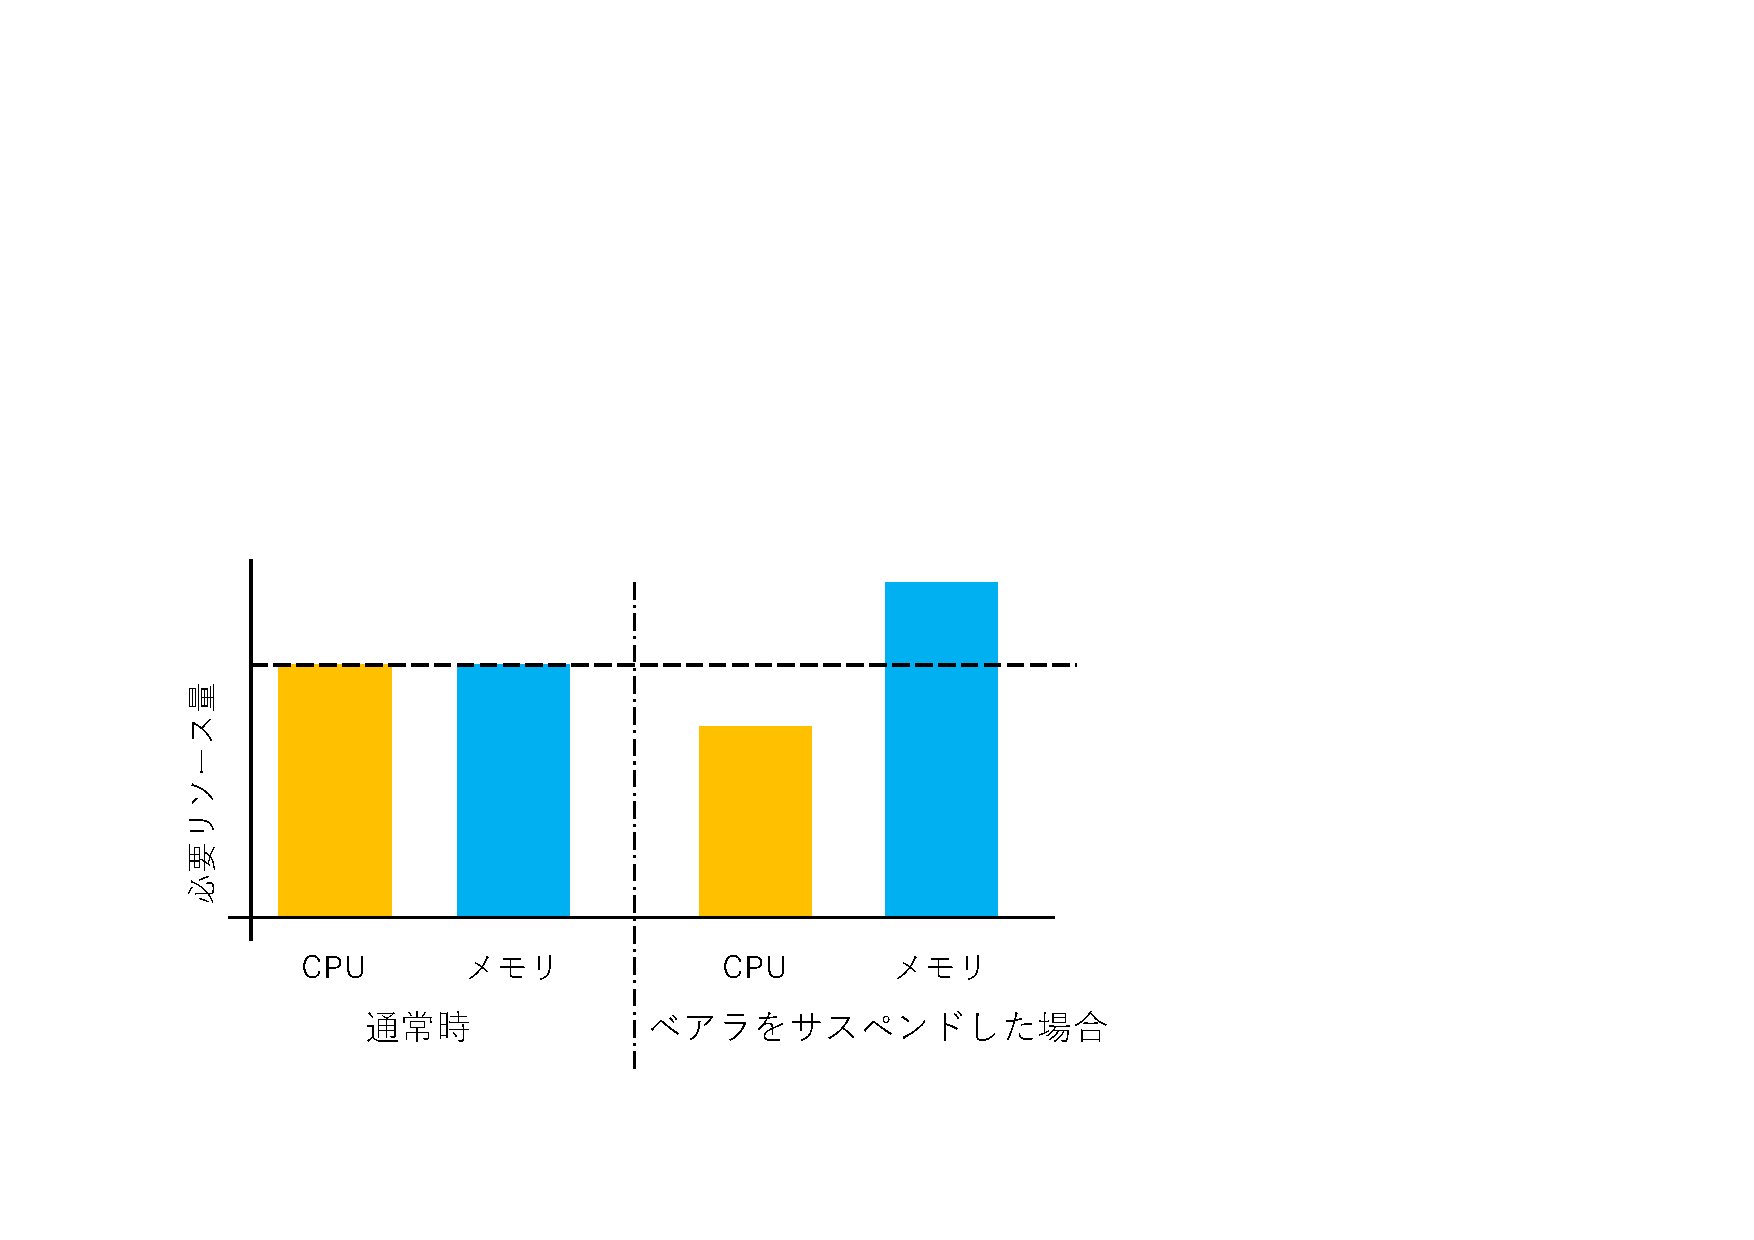
\includegraphics[width=0.7\hsize]{グラフ.pdf}
  \caption{負荷のオフロード}
	\label{グラフ}
\end{figure}
\subsection{説明}
図\ref{detach-ON}は、M2M/IoT端末が最初にネットワークに接続した際の様子を示す。通常通り、アタッチの処理を行い、ベアラを確立する。図\ref{detach-OFF}は、M2M/IoT端末がネットワークから切断された際の様子を示す。通常と異なり、デタッチ処理が行われないため、ベアラはそのまま維持される(UE-eNodeB間の無線帯域は解放される)。図\ref{detach-reON}はM2M/IoT端末が再びネットワークに接続した時の様子を示す。この場合、以前使用したベアラが残っているため、M2M/IoT端末はアタッチ処理をスキップしてデータの送受信を開始できる。

\begin{figure}[htbp]
	\centering
	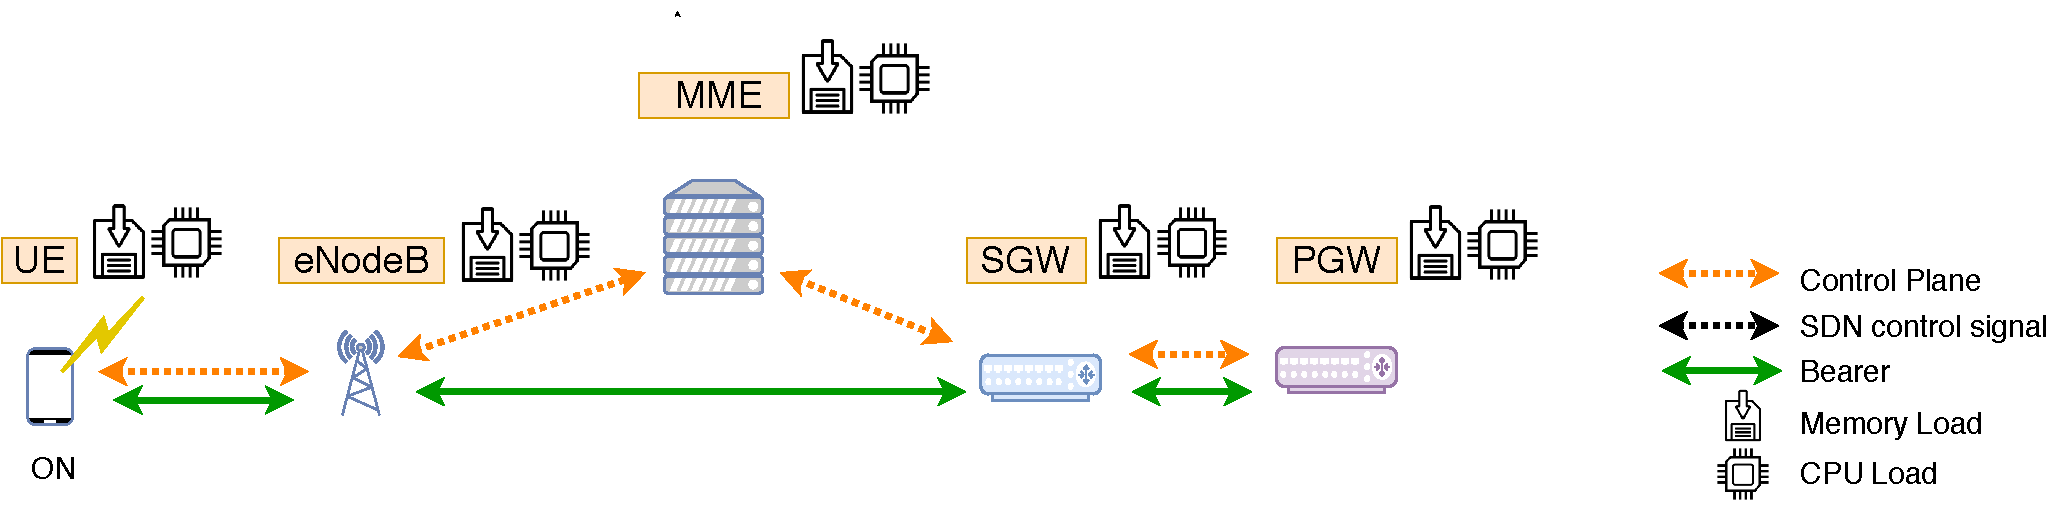
\includegraphics[width=0.7\hsize]{detach-ON.pdf}
  \caption{端末が最初にネットワークに接続した時と処理}
	\label{detach-ON}
\end{figure}

\begin{figure}[htbp]
	\centering
	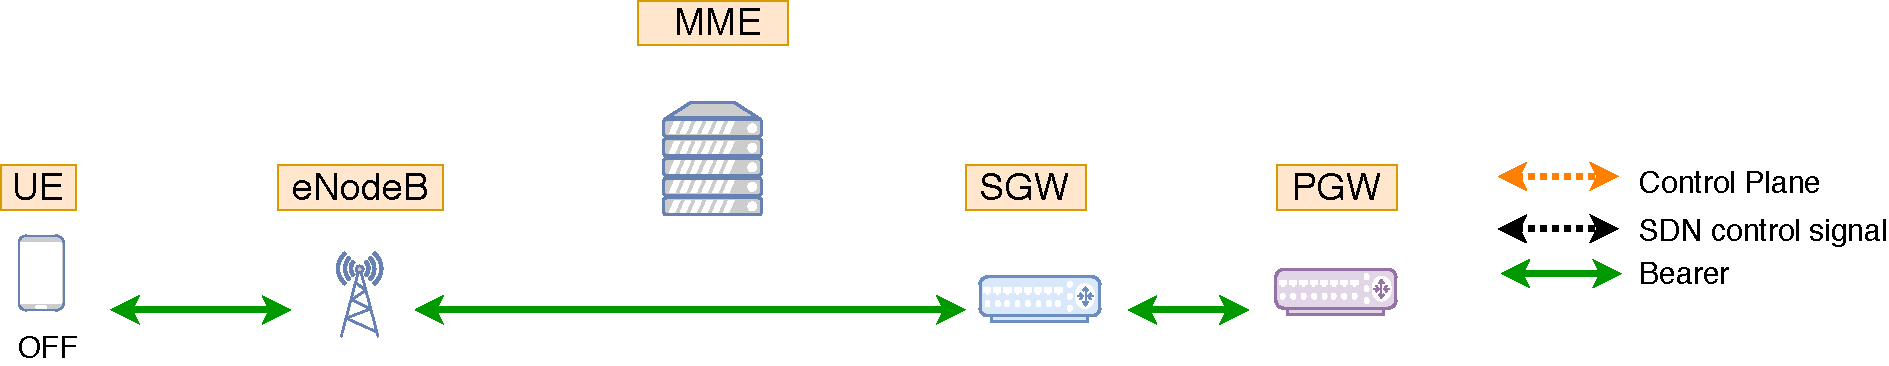
\includegraphics[width=0.7\hsize]{detach-OFF.pdf}
  \caption{端末がネットワークから切り離された時の処理}
	\label{detach-OFF}
\end{figure}

\begin{figure}[htbp]
	\centering
	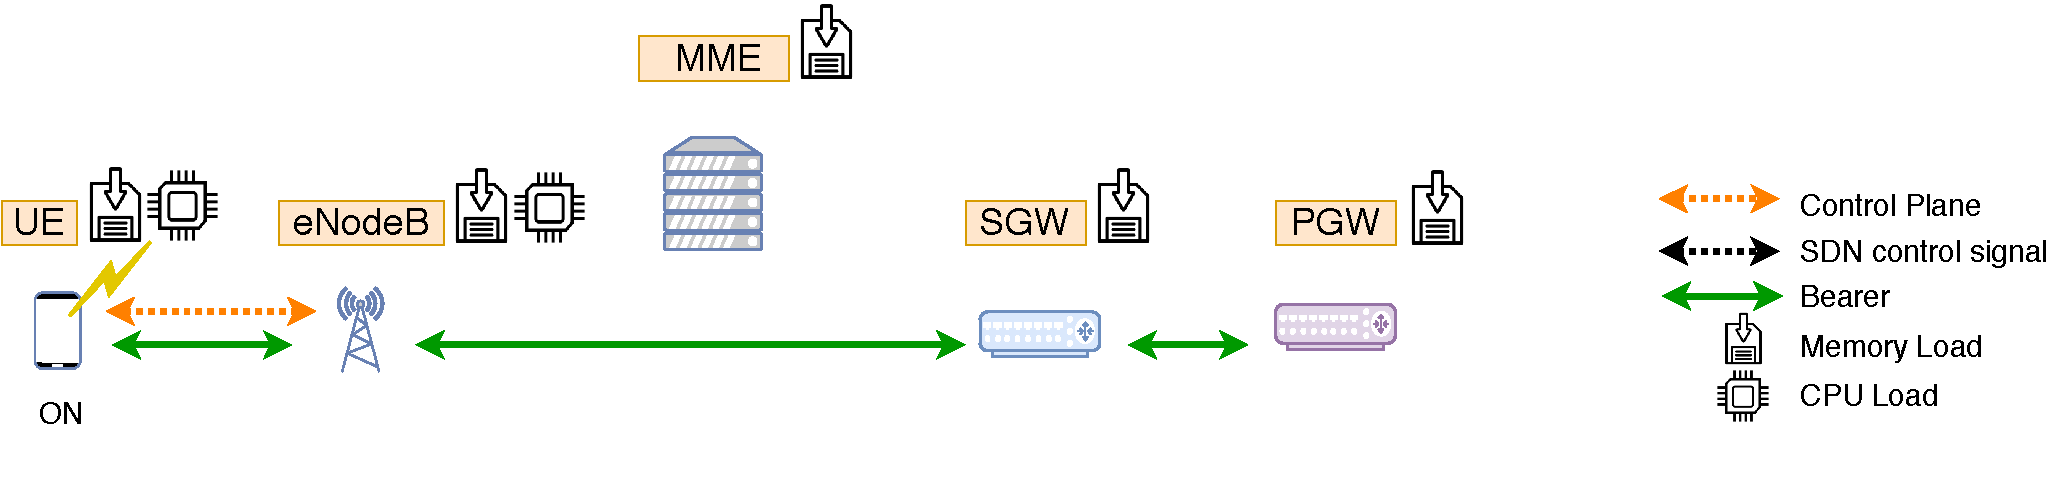
\includegraphics[width=0.7\hsize]{detach-reON.pdf}
  \caption{端末が2回目以降にネットワークに接続した時の処理}
	\label{detach-reON}
\end{figure}

% \clearpage
% eNodeB、MME、SGWおよびPGWは、ネットワークに接続されていないM2M/IoT端末のセッション情報を保持する必要があるため、リソース(主にメモリ)が圧迫されることが予想される。また、場合によっては、端末に割り当てるIPアドレスの枯渇などが発生する可能性もある。そのような、事態が発生した場合は、セッション情報がもっとも古い端末(最後にデータを送受信したタイミングが最も古い端末)から優先的にデタッチ処理を行い、リソースを解放する。

% \subsection{利点}
% 上述の方法で、アタッチ処理を行う回数を減らすことで、M2M/IoT端末によるコントロールプレーンの負荷の増大に対して、根本的でかつ効果的な対策ができるのではないかと思う。負荷の原因そのものを削減できる点は、負荷分散などの他の方式と比較した際に強みであると思う。


%
% \section{今後の予定}
%
% \begin{itemize}
%   \item I/O待ち時間の調査を行う。具体的には先行研究論文や富士通株式会社などが公開しているサーバパフォーマンスに関するホワイトペーパーなどを参考にする。
% 	% \item PCRFの配置および課金処理の実現方法についての調査。
% \end{itemize}

\section*{\addcontentsline{toc}{section}{参考文献}}
{\scriptsize
\bibliographystyle{IEEEtran}
\bibliography{/Users/t-adachi/Documents/study/Bibliography/bib/hpt_core_network/myBib/LABbiblio,/Users/t-adachi/Documents/study/Bibliography/bib/hpt_core_network/Study_Group_Bibtex/bib/hptCoreNetwork_Study}
}
\end{document}
